% Source - https://tex.stackexchange.com/a/728329

\documentclass[tikz]{standalone}
\usetikzlibrary{arrows.meta, nfold, decorations.markings}
\makeatletter
\tikzset{
    offset/.code=\tikz@addmode{
        \pgfgetpath\tikz@temp
        \pgfsetpath\pgfutil@empty
        \pgfoffsetpath\tikz@temp{#1}
    }
}
\makeatother
\begin{document}
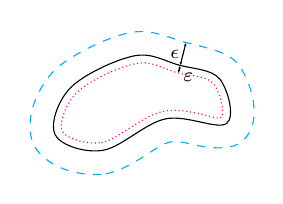
\begin{tikzpicture}
    \draw[
        postaction={draw=cyan, dashed, offset=+-3mm},
        postaction={draw=magenta, densely dotted, offset=+1mm},
        decoration={
            name = markings,
            mark = at position 0.5 with {
                \draw[arrows={[scale=.25]}, Latex-Latex] 
                (0,0) -- node[node font=\scriptsize, inner sep=+.15em, left] {$\epsilon$} (down:3mm);
                \draw[arrows={[scale=.25]}, Latex-Latex] 
                (0,0) -- node[node font=\scriptsize, inner sep=+.15em,below right] {$\varepsilon$} (up:1mm);
            }
        },
        postaction=decorate,
    ] plot [smooth cycle, tension=0.6] coordinates {
        (4.4,0.4) 
        (5,0.2) 
        (5.8,0.6) 
        (6.5773,0.5421)
        (6.4905,1.1074) 
        (5.9752,1.2828) 
        (5.4,1.4) 
        (4.6,1) 
    };
\end{tikzpicture}
\end{document}
